\documentclass[12pt,a4paper]{amsart}

\synctex = 1

\DeclareMathAlphabet{\mathpzc}{OT1}{pzc}{m}{it}

\def\Bb{\mathbb{B}}
\def\C{\mathbb{C}}
\def\E{\mathbb{E}}
\def\F{\mathbb{F}}
\def\Hh{\mathbb{H}}
\def\K{\mathbb{K}}
\def\N{\mathbb{N}}
\def\P{\mathbb{P}}
\def\Q{\mathbb{Q}}
\def\R{\mathbb{R}}
\def\Z{\mathbb{Z}}



%A
\DeclareMathOperator{\akte}{akte}
%B
\DeclareMathOperator{\bearbeitet}{bearbeitet}
\DeclareMathOperator{\Black}{Black}
%C
%D
\DeclareMathOperator{\deff}{def}
\DeclareMathOperator{\Dom}{Dom}
%E
\DeclareMathOperator{\Einbruch}{Einbruch}
\DeclareMathOperator{\ermittler}{ermittler}
\DeclareMathOperator{\ext}{ext}
%F
%G
\DeclareMathOperator{\gdw}{gdw}
%H
%I
%J
%K
%L
\DeclareMathOperator{\wle}{le}
\DeclareMathOperator{\ltdermittler}{ltdermittler}
%M
\DeclareMathOperator{\Mulder}{Mulder}
%N
\DeclareMathOperator{\Name}{Name}
%O
\DeclareMathOperator{\offen}{offen}
%P
\DeclareMathOperator{\Pathologie}{Pathologie}
%Q
%R
%S
\DeclareMathOperator{\Skinner}{Skinner}
\DeclareMathOperator{\Skully}{Skully}
\DeclareMathOperator{\Sonderermittler}{Sonderermittler}
%T
%U
%V
%X
%Z

\def\fspace{\rule{0.5cm}{0cm}}
\theoremstyle{definition}
\newtheorem{aufgabe1}{Aufgabe}

\usepackage{amsmath,amsthm,amssymb}
\usepackage[utf8]{inputenc}
\usepackage{wasysym}
\usepackage{stmaryrd}
\usepackage{nicefrac}
\usepackage{listings}
\usepackage{pictex}
\usepackage{color}
\usepackage{graphicx}
\usepackage{german}

\lstset{basicstyle=\small}

%%%%%%%%%%%%%%%%%%%%%%%%%%%%%%%%%%%%%%%%%%%%%%%%%%%%%%%%%%%%%%%%%%%%%%%

\begin{document}

\title{Blatt 6}

\author{Daniel Schmidt \& Pamela Fleischmann}

\maketitle

\begin{aufgabe1}

Die Methode \texttt{reachable} lässt sich wie folgt implementieren: \\

\lstinputlisting{code/a1.P}

Ein Aufruf würde beispielsweise so aussehen: \\

\begin{lstlisting}
ready>>consult(kante.T).
ready>>consult(a1.P).
ready>>reachable(g1, "A", ["y"], Z).
CORAL::error : Not in insert mode !
ready>>?reachable(g1, "A", ["y"], Z).
Z="B".
        ... next answer ? (y/n/all)[y]
y
Z="K".
        ... next answer ? (y/n/all)[y]y
Z="C".
        ... next answer ? (y/n/all)[y]y
Z="D".
        ... next answer ? (y/n/all)[y]y
Z="E".
        ... next answer ? (y/n/all)[y]y
Z="L".
        ... next answer ? (y/n/all)[y]y
Z="F".
        ... next answer ? (y/n/all)[y]y
Z="G".
        ... next answer ? (y/n/all)[y]y
Z="J".
        ... next answer ? (y/n/all)[y]all
Z="I".
Z="H".
(Number of Answers = 11)
ready>>?reachable(g1, "A", [1,1], Z).
Z="B".
        ... next answer ? (y/n/all)[y]y
Z="K".
        ... next answer ? (y/n/all)[y]y
Z="D".
        ... next answer ? (y/n/all)[y]y
Z="E".
        ... next answer ? (y/n/all)[y]y
(Number of Answers = 4)
\end{lstlisting}

\end{aufgabe1}

\begin{aufgabe1}
Betrachte folgendes Datalog-Programm:\\
$p(a,b,c,d,e,f). p(a,a,b,b,c,c). p(a,a,a,b,b,c). p(c,c,c,b,b,a).$\\
$r_1= q(U,V,W,X,Y,Z) :- p(U,V,W,X,Y,Z).$\\
$r_2=q(U,V,W,X,Y,Z) :- q(Z,U,V,W,X,Y).$\\
$r_3=q(X,Y,Z,U,V,W) :- q(U,V,X,W,Y,Z), q(W,Y,Z,U,V,X).$\\
$r_4=r(X,Y,Z) :- q(X,Y,X,Z,X,Y).$\\
Sei weiter $r(a,b,c)$ ein Ziel. Dann hat ein Beweisbaum zu $r(a,b,c)$ die folgende Form
\begin{center}
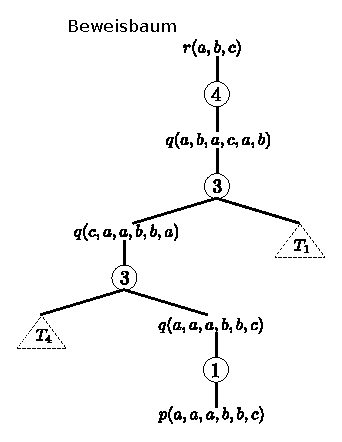
\includegraphics[]{tree.eps}
\end{center}
mit den Unterbäumen
\begin{center}
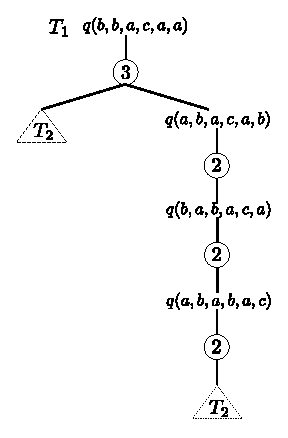
\includegraphics[]{t1.eps} 
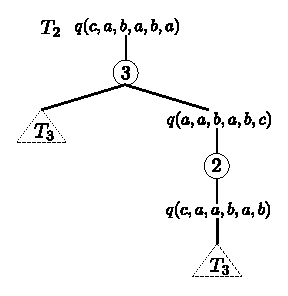
\includegraphics[]{t2.eps}
\end{center}
\begin{center}
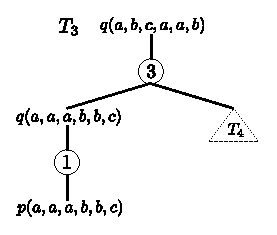
\includegraphics[]{t3.eps}
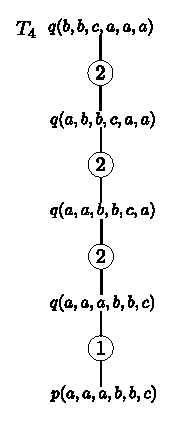
\includegraphics[]{t4.eps}
\end{center}
Für das Beweismuster kann jedes $a$ durch ein $X$, jedes $b$ duch ein $Y$ und jedes $c$ durch ein $Z$ ersetzt werden. Eine Umbennung von Variablen im Beweismuster
ist nicht nötig, da im Rumpf der Regeln keine neuen Variablen eingeführt werden, sondern alle Variablen in den Rümpfen auch in den zugehörigen Köpfen vorkommen.
\end{aufgabe1}


\begin{aufgabe1}
Das Programm sieht so aus:
\lstinputlisting[caption=a3.P]{code/a3.P}

Die zugehörtige Table file die zuerst importiert werden muss so:
\lstinputlisting[caption=a3.T]{code/a3.T}

Die Sprache ist definiert als: $L=hello(hello | test | world)^{\ast}world$ (wobei das ``|'' Symbol für oder steht).

Eine Ausgabe dieses Programms ist hier zu sehen:

\lstinputlisting[caption=a3.log]{code/a3.log}

\end{aufgabe1}

\end{document}
